\chapter{Two-Stage Pre-training Method for Medical Vision and Language Task}
\label{chapter:ch3}

In this chapter, we will provide a detailed explanation of the method proposed in our research. Initially, we will discuss two problems that arise when directly applying vision-language pre-training in the medical domain (Sec.~\ref{Problems}). We will then introduce our proposed method (Sec.~\ref{Method}), which aims to address these issues. The subsequent section will explore into the network architecture, layers, and components utilized in our approach (Sec.~\ref{Architecture}). Furthermore, we will focus on the training pipeline (Sec.~\ref{training}) that consists of fist stage pre-training and second stage pre-training. The first stage pre-training (Sec.~\ref{Stageone})is where the model acquires essential organ-specific knowledge. We will elaborate on the methodology employed for image segmentation and its contribution to a comprehensive understanding of organ structures. In the second stage of pre-training (Sec.~\ref{Stagetwo}), we will explain the original vision-language pre-training procedure that employs medical images and captions. Additionally, we will demonstrate the datasets utilized in our experiments (Sec.~\ref{Dataset}) and explore the process of generating a dataset for the first-stage pre-training (Sec.~\ref{Gencaption}).

\section{Problems in Medical Vision-Language Pre-training}
\label{Problems}
The latest advanced models in medical visual question answering use a two-step approach called pre-training and fine-tuning \cite{chen2022align, chen2023towards, moon2022multi, yan2022clinical, chen2022multi, Wang2022MedCLIPCL}. However, when applying the vision-language pre-training technique in the medical domain, we encounter two significant challenges. The first challenge arises from the scarcity of data available for pre-training (Sec.~\ref{Shortage}). The second challenge relates to the model's lack of fundamental knowledge about medical organs (Sec.~\ref{Lackknowledge}).

\subsection{Shortage of Data}
\label{Shortage}
The first problem is the shortage of data during pre-training. Vision-language pre-training technique relies on a large-scale datasets of image-text pairs for successful learning. However, in the medical domain, the availability of such datasets is limited. Typically, in the medical domain, we have around 300K image-caption pairs \cite{subramanian-2020-medicat}, but pre-training techniques require approximately 4 million image-caption pairs for effective learning \cite{li2021align}. This scarcity of data in the medical domain can be attributed to privacy concerns and the complexity of annotating medical images, which require expert physicians to provide accurate captions. Acknowledging the difficulty and resource-intensive nature of collecting additional image-caption dataset pairs, we have chosen to set this aside and proceed with addressing the next problem. However, we believe our proposed method can work well in the low data regime.

\subsection{Model's Lack of Organ Knowledge}
\label{Lackknowledge}
The second problem is, during pre-training, the model lacks fundamental knowledge about organs, such as their size, shape, and location. The rationale behind this problem is that medical images consistently depict the same group of organs: see Figure~\ref{fig:reasonsOfProblem}(a), and captions primarily focus on describing individual organs; see Figure~\ref{fig:reasonsOfProblem}(b). Consequently, during the pre-training phase, the model faces difficulty in accurately identifying the relevant image region corresponding to the caption. For instance, in Figure~\ref{fig:probelm}, with a caption that focuses solely on one organ (liver) in an image containing multiple organs,  the model struggle to identify the specific regions (such as the green, red, yellow, or purple areas) that represent the liver in the visual representation. Additionally, in Figure~\ref{fig:probelmMLM}, the model faces challenges in tasks such as filling in masked words during masked language modeling pre-training due to its limited understanding of the visual appearance of healthy organs. Even when provided with choices such as liver, spleen, or kidneys, the model still struggles to accurately identify the organ in masked words. It is crucial to provide the model with fundamental organ knowledge prior to the original pre-training stage.

\begin{figure}[t]
\begin{center}
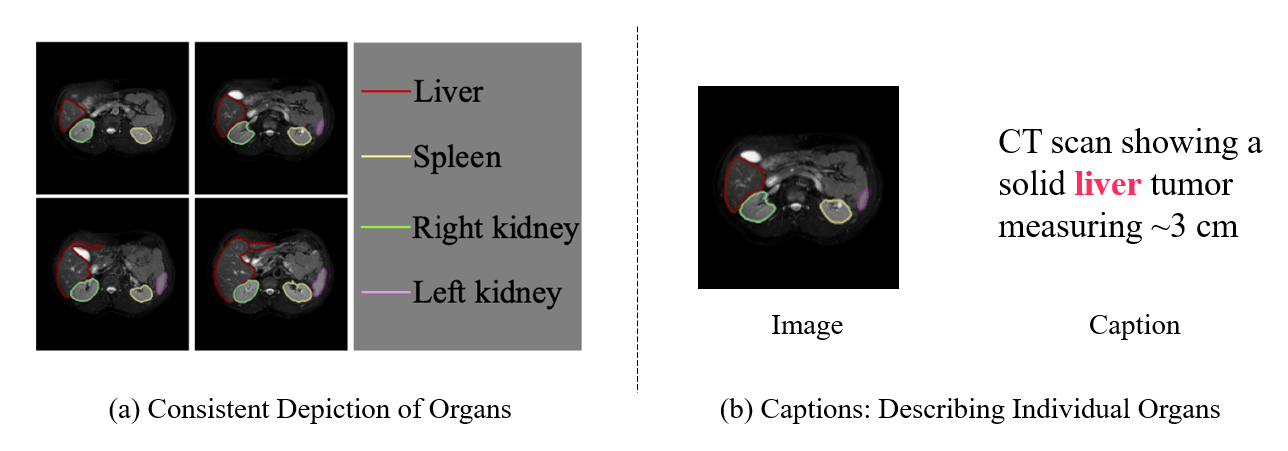
\includegraphics[width=1.0\linewidth]{Chapter_3/chap3_reasonOfProblem.png}
\end{center}
   \caption{Two reasons behind the model's lack of organ knowledge. (a) clearly illustrates four abdominal images, each showcasing the consistent presence of organs such as the liver, spleen, and kidneys \cite{chen2022c}. In (b), the abdomen is illustrated, and the corresponding caption specifically describes the liver while disregarding the other organs present.
}
\label{fig:reasonsOfProblem}
\end{figure}

\begin{figure}[t]
\begin{center}
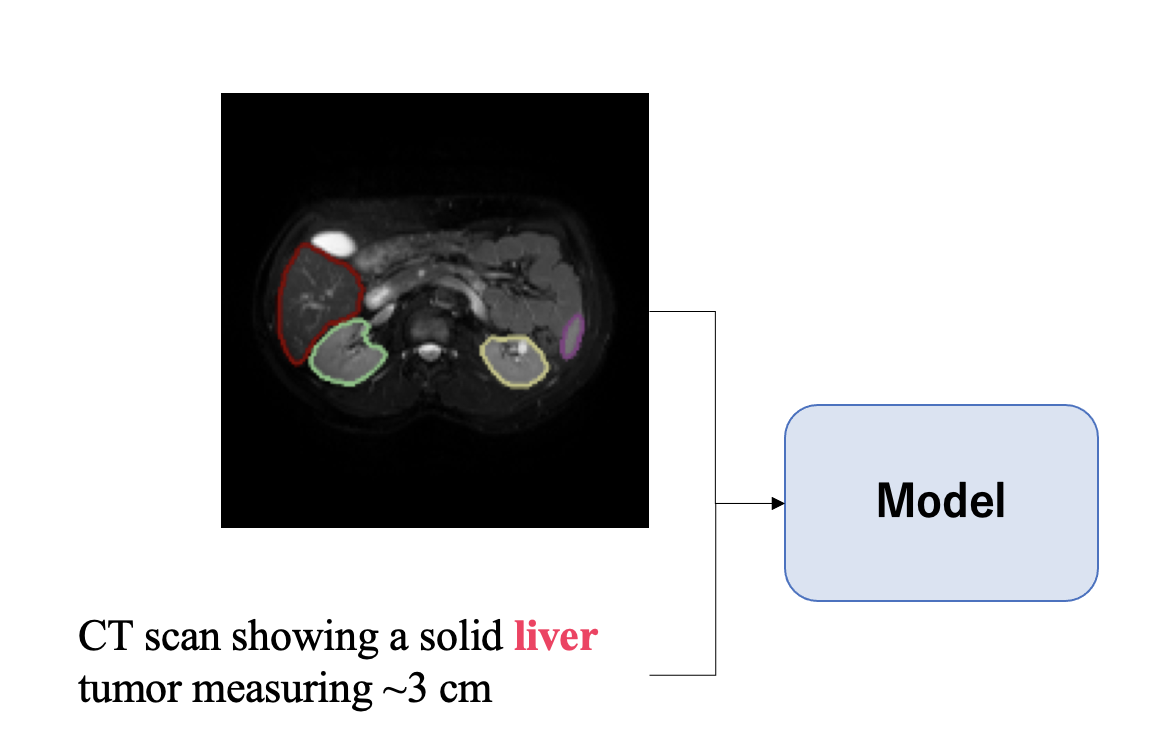
\includegraphics[width=1.0\linewidth]{Chapter_3/chap3_problem.png}
\end{center}
   \caption{Challenge in the application of vision-language pre-training in the medical domain \cite{chen2022c}: The model struggles to identify the specific regions (such as the green, red, yellow, or purple areas) that represent the liver in the visual representation. 
}
\label{fig:probelm}
\end{figure}

\begin{figure}[t]
\begin{center}
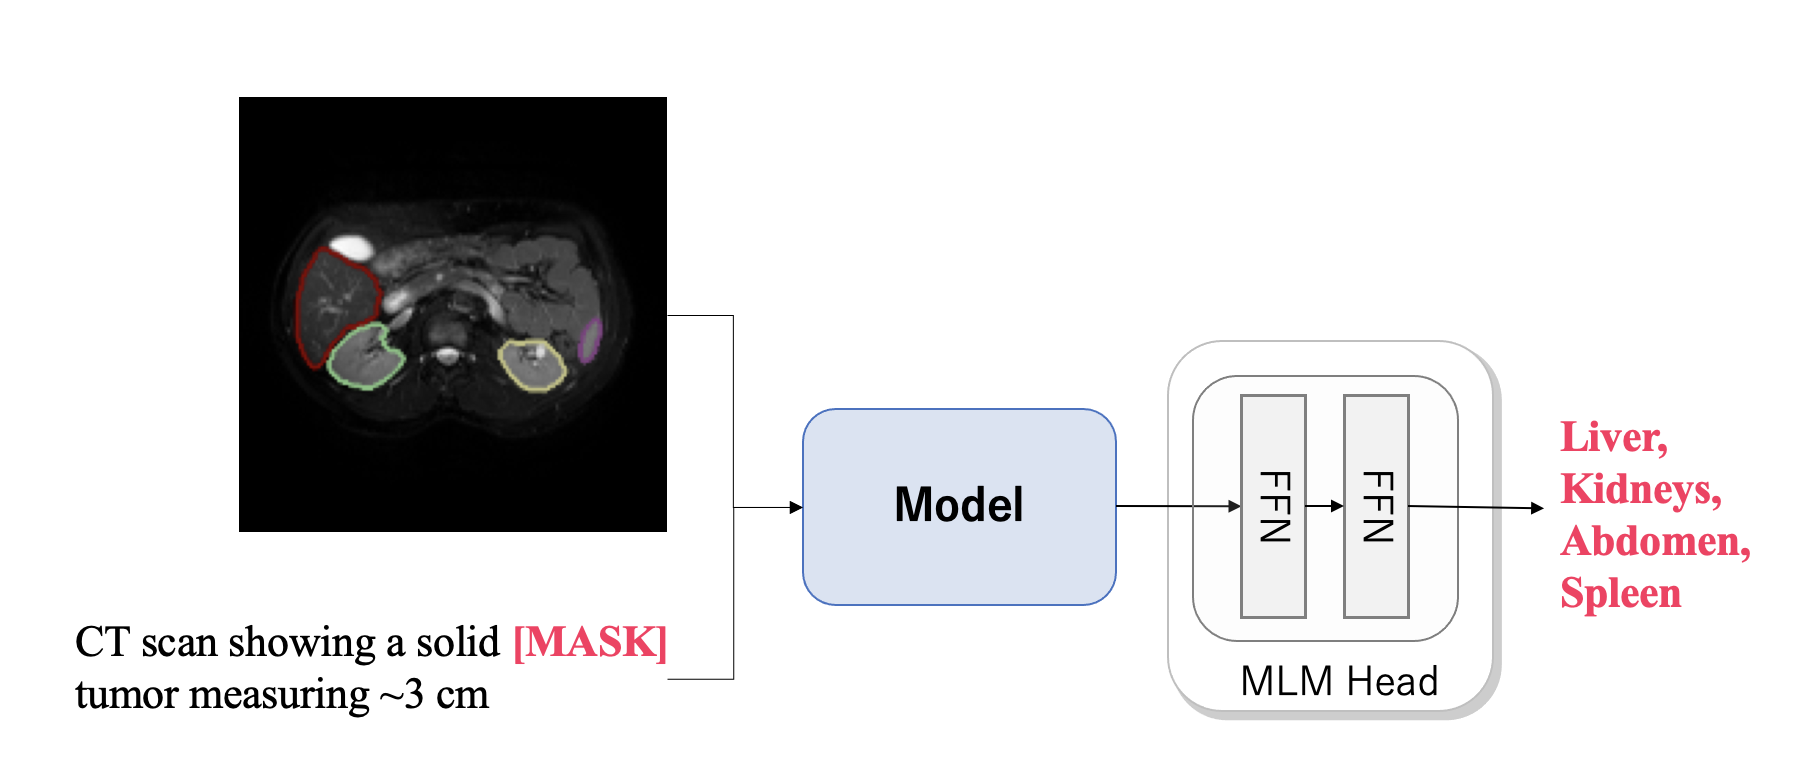
\includegraphics[width=1.0\linewidth]{Chapter_3/chap3_problemMLM.png}
\end{center}
   \caption{Challenge in the application of vision-language pre-training in the medical domain \cite{chen2022c}, especially in masked language modeling: The model encounters challenges in tasks such as filling masked words during pre-training due to its limited knowledge of the visual appearance of healthy organs. Despite being provided with choices such as liver, spleen, or kidneys, accurately identifying the organ in masked words remains a difficult task.
}
\label{fig:probelmMLM}
\end{figure}

\section{Proposed Method}
\label{Method}
In order to address the aforementioned challenge, this thesis proposes a two-stage pre-training approach aimed at equipping the model with fundamental organ knowledge prior to the original pre-training stage. More specifically, we undertake the pre-training process in two separate stages, in contrast to previous approaches \cite{chen2022multi, chen2022align} that utilized only one stage. Figure~\ref{fig:proposedPretrainStep} provides a visualization of the pre-training steps involved in our proposed method.

The first stage involves the use of an medical image segmentation \cite{ronneberger2015u} task to acquire important and fundamental organ knowledge, while utilizing captions as input to facilitate a comprehensive understanding of organ structures within medical images; see Figure~\ref{fig:proposedPretrainStep}(a). By incorporating this stage, the model gains a foundational understanding of medical organ concepts that is often lacking in previous work. In the second stage, the original vision-language pre-training process is performed using the medical images and captions: see Figure~\ref{fig:proposedPretrainStep}(b). The objective of the two-stage pre-training methodology is to enhance the model's understanding of medical concepts and improve the quality of multimodal representations.

Medical image segmentation is a crucial task in the field of medical imaging analysis. It involves identifying and outlining different structures or regions within medical images, like organs, tumors, or lesions; see Figure~\ref{fig:segment}. Accurate segmentation is vital for various clinical applications, such as diagnosis, treatment planning, and disease monitoring. By performing medical image segmentation, the model gains an understanding of various aspects of organs, such as their shapes and positions within the image. This process enables the model to acquire essential knowledge about organs and their characteristics.

\begin{figure}[t]
\begin{center}
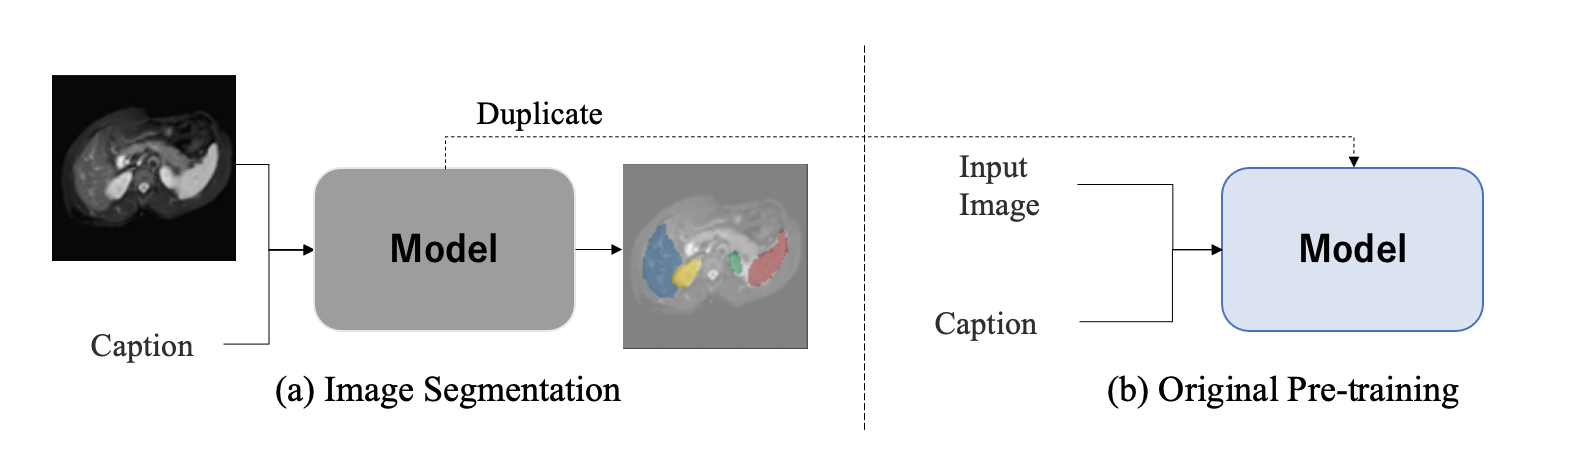
\includegraphics[width=1.0\linewidth]{Chapter_3/chap3_proposedPretrainStep.png}
\end{center}
   \caption{The pre-training process comprises two stages: (a) stage one focuses on a segmentation task \cite{kavur2021chaos}, while (b) stage two adheres to the original pre-training methodology. 
}
\label{fig:proposedPretrainStep}
\end{figure}

\begin{figure}[t]
\begin{center}
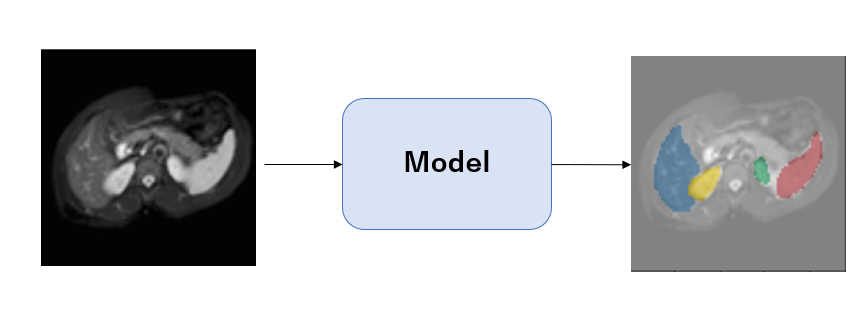
\includegraphics[width=1.0\linewidth]{Chapter_3/chap3_segmen.png}
\end{center}
   \caption{Medical image segmentation \cite{kavur2021chaos} 
}
\label{fig:segment}
\end{figure}

\section{Model Architecture}
\label{Architecture}
The model architecture employed in this thesis builds upon previous research on vision-language pre-training models \cite{Dou_2022_CVPR}, incorporating three key components: the image encoder, text encoder, and fusion encoder. The image encoder focuses on mapping an image into its corresponding image representation, while the text encoder aims to map textual input into a text representation. The fusion encoder plays a crucial role in integrating the image and text representations. In the first stage of pre-training, we introduce a segmentation head to the model, specifically positioned after the fusion encoder. In the second stage of pre-training, we incorporate a Masked-Language Modeling Head and an Image-Text Matching Head into the model. During the fine-tuning phase, we incorporate a Visual Question Answering (VQA) head to perform VQA tasks. Further details regarding each architectural component will be provided in the subsequent sections. Figure~\ref{fig:modelArchitecture} shows an overview of the architecture. 

\begin{figure}[t]
\begin{center}
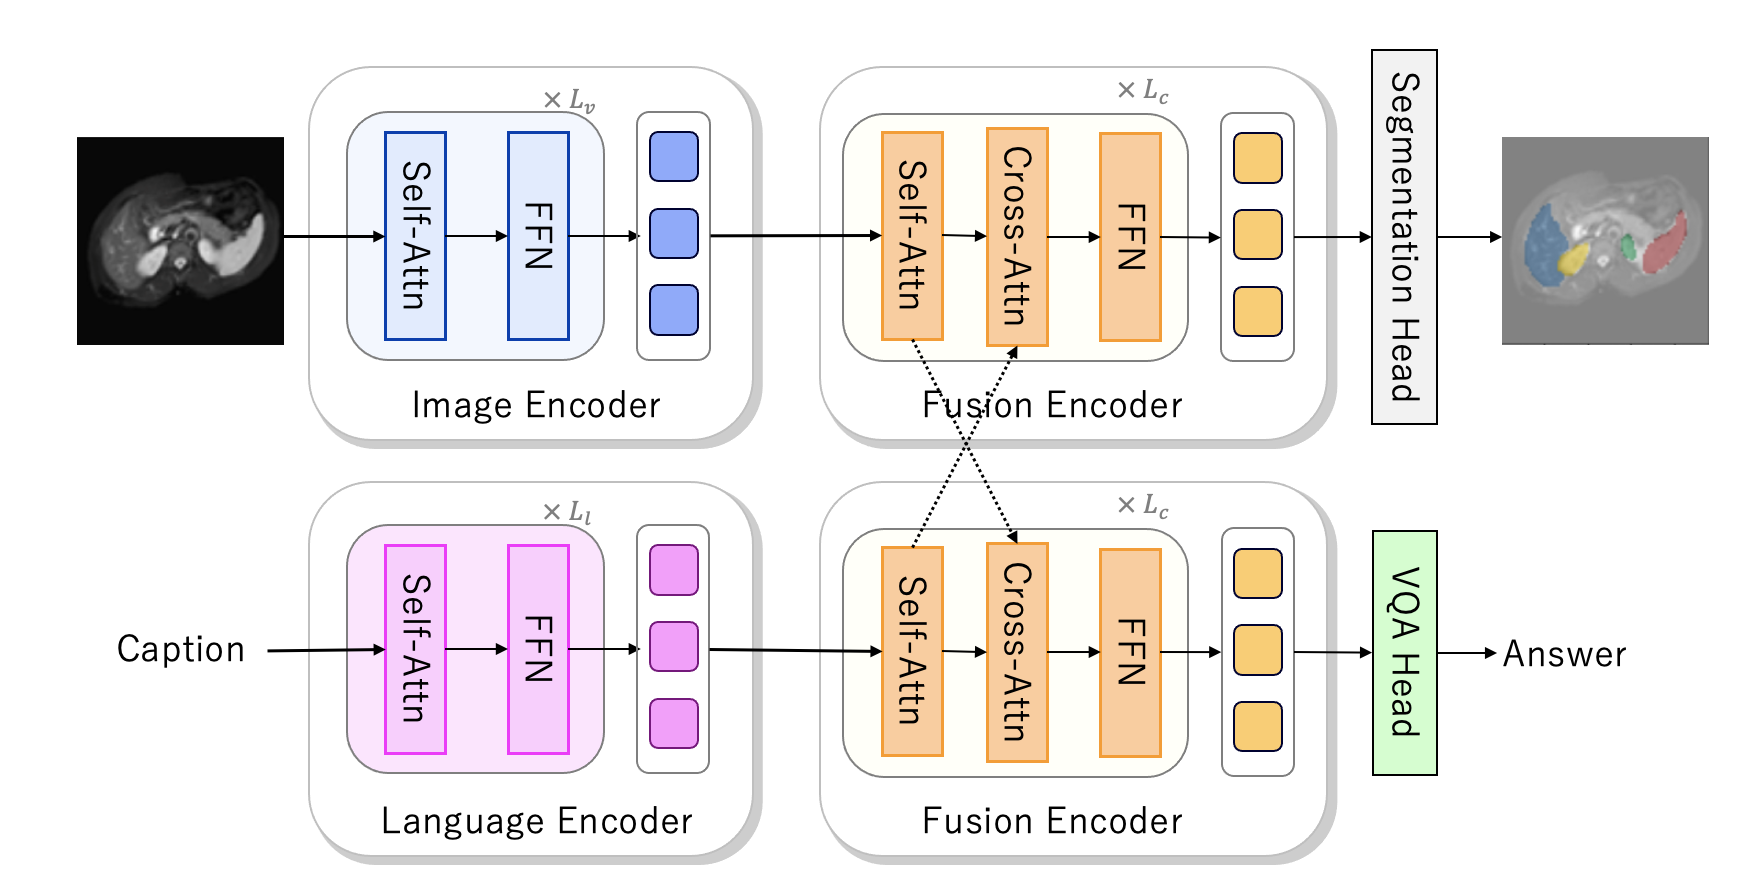
\includegraphics[width=1.0\linewidth]{Chapter_3/chap3_model.png}
\end{center}
   \caption{Overview of the architecture of the proposed method. The component of the image is from paper \cite{kavur2021chaos}.
}
\label{fig:modelArchitecture}
\end{figure}

% For our thesis, we utilize the Vision Transformer pre-trained on the CLIP (ViT-16) as the image encoder. The text encoder is based on the BERT model, renowned for its proficiency in language understanding tasks. The fusion encoder follows the Transformer architecture. It is worth noting that alternative models can be employed as the image and text encoders, provided they can effectively map the respective inputs into their respective representations. Throughout the experimental section, we also explore the substitution of the image encoder with various other models to facilitate a more comprehensive evaluation. To facilitate image segmentation in the first stage of pre-training, a segmentation head is added to the model, specifically after the fusion encoder in the image part. Furthermore, for the second stage pre-training, we add a Masked-Language Modeling Head and an Image-Text Matching Head to the model. During fine-tuning, we introduce a Visual Question Answering (VQA) head to enable VQA tasks. Further details regarding each architectural component will be provided in the subsequent sections.

{\bf Image Encoder:} 
The image encoder is responsible for mapping the image input to its corresponding image representation. In this thesis, we employ the ViT architecture \cite{dosovitskiy2020vit} that has been pre-trained using the CLIP \cite{radford2021learning}, specifically ViT/16. The input image is transformed into a sequence of embeddings, denoted as $\{v_{cls},v_{1}, ...,v_{N}\}$, where $v_{cls}$ represents the embedding of the $[CLS]$ token. The image encoder can be instantiated with various models capable of transforming high-resolution images into their corresponding image representations, for instance, ResNet \cite{He_2016_CVPR} and Swin Transformer \cite{Liu_2021_ICCV}. The exploration of different image encoder setups will be elaborated upon in Chapter \ref{chapter:ch4}.

{\bf Text Encoder:} 
The text encoder converts the text input into its corresponding text representation. In this thesis, we use RoBERTa \cite{zhuang-etal-2021-robustly} as the chosen model for the text encoder. Specifically, the text encoder takes an input text T and transforms it into a sequence of embedding $\{w_{cls},w_{1}, ...,w_{N}\}$. The text encoder is initialized with the weights of the RoBERTa model, which provides a strong foundation for text representation learning. 

{\bf Fusion Encoder:} 
The fusion encoder plays a crucial role in combining the image and text representations, allowing the model to learn and understand both visual and textual information effectively. In this thesis, we use a fusion encoder called the dual fusion encoder, which is based on the Transformer architecture \cite{vaswani2017attention}. As shown in Figure~\ref{fig:modelArchitecture}, the fusion encoder is incorporated into the model following the image encoder and text encoder modules. It consists of three layers: the self-attention layer, the cross-attention layer, and the feed-forward neural networks layer (FFN). The cross-attention layer is where the fusion of the image and text representations occurs. Within the fusion encoder, positioned subsequent to the text encoder, the image representation assumes the role of key and value inputs for cross-attention. Conversely, the self-attention output derived from the text representation serves as the query. Similarly, in the image fusion encoder, the roles are reversed, with the image representation serving as the query and the text representation acting as the key and value inputs. This allows for effective fusion and interaction between the image and text modalities, enhancing the model's multimodal understanding and representation.

{\bf Segmentation Head:}
In order to facilitate image segmentation during pre-training stage one, a segmentation head is integrated into the model by connecting it to the image fusion encoder. The segmentation head consists of a block of convolutional layers, the ReLU activation function, batch normalization layers, and a convolutional up-sampling layer, following the design principles outlined in the U-Net paper \cite{ronneberger2015u}. 

{\bf Masked-Language Modeling Head:}
To address the masked-language modeling task in the second stage of pre-training, we integrate a masked-language modeling head into our model. It is positioned after the text fusion encoder. It consists of two layers of feed-forward neural network (FFN).

{\bf Image-Text Matching Head:}
To facilitate the image-text matching task in the second stage of pre-training, our model is integrated with an image-text matching head. This head consists of two layers of feed-forward neural network (FFN) and is positioned after the text fusion encoder.

{\bf VQA Head:}
To enable visual question answering in our model, we incorporate a VQA head after the fusion encoder. The VQA head involves two Feed Forward Neural Network layers. Following previous work \cite{chen2022align, chen2022multi}, we consider VQA as a classification task, the output layer is designed with a size corresponding to the number of candidate answers. This VQA head enables our model to generate responses to questions by leveraging its comprehensive understanding of the multimodal inputs.

\section{Training Pipeline}
\label{training}
 As illustrated in Figure~\ref{fig:compare}(b), the model represents the complete pipeline used in this work, consisting of three main stages. The first stage involves pre-training with an image segmentation task, where the model learns to identify and delineate organ structures in medical images. This initial pre-training stage is followed by the second stage, which is vision-language pre-training. During this stage, the model is trained to understand the relationship between medical images and corresponding textual information. Finally, the model undergoes finetuning specifically for the visual question answering task.

It is worth noting that this approach differs from previous work, as highlighted in Figure~\ref{fig:compare}(a), where the first stage of pre-training was not incorporated. In the subsequent section, a detailed explanation of both pre-training stage one (\ref{Stageone}) and pre-training stage two (\ref{Stagetwo}) will be provided, exploring their respective methodologies and objectives.

\begin{figure}[t]
\begin{center}
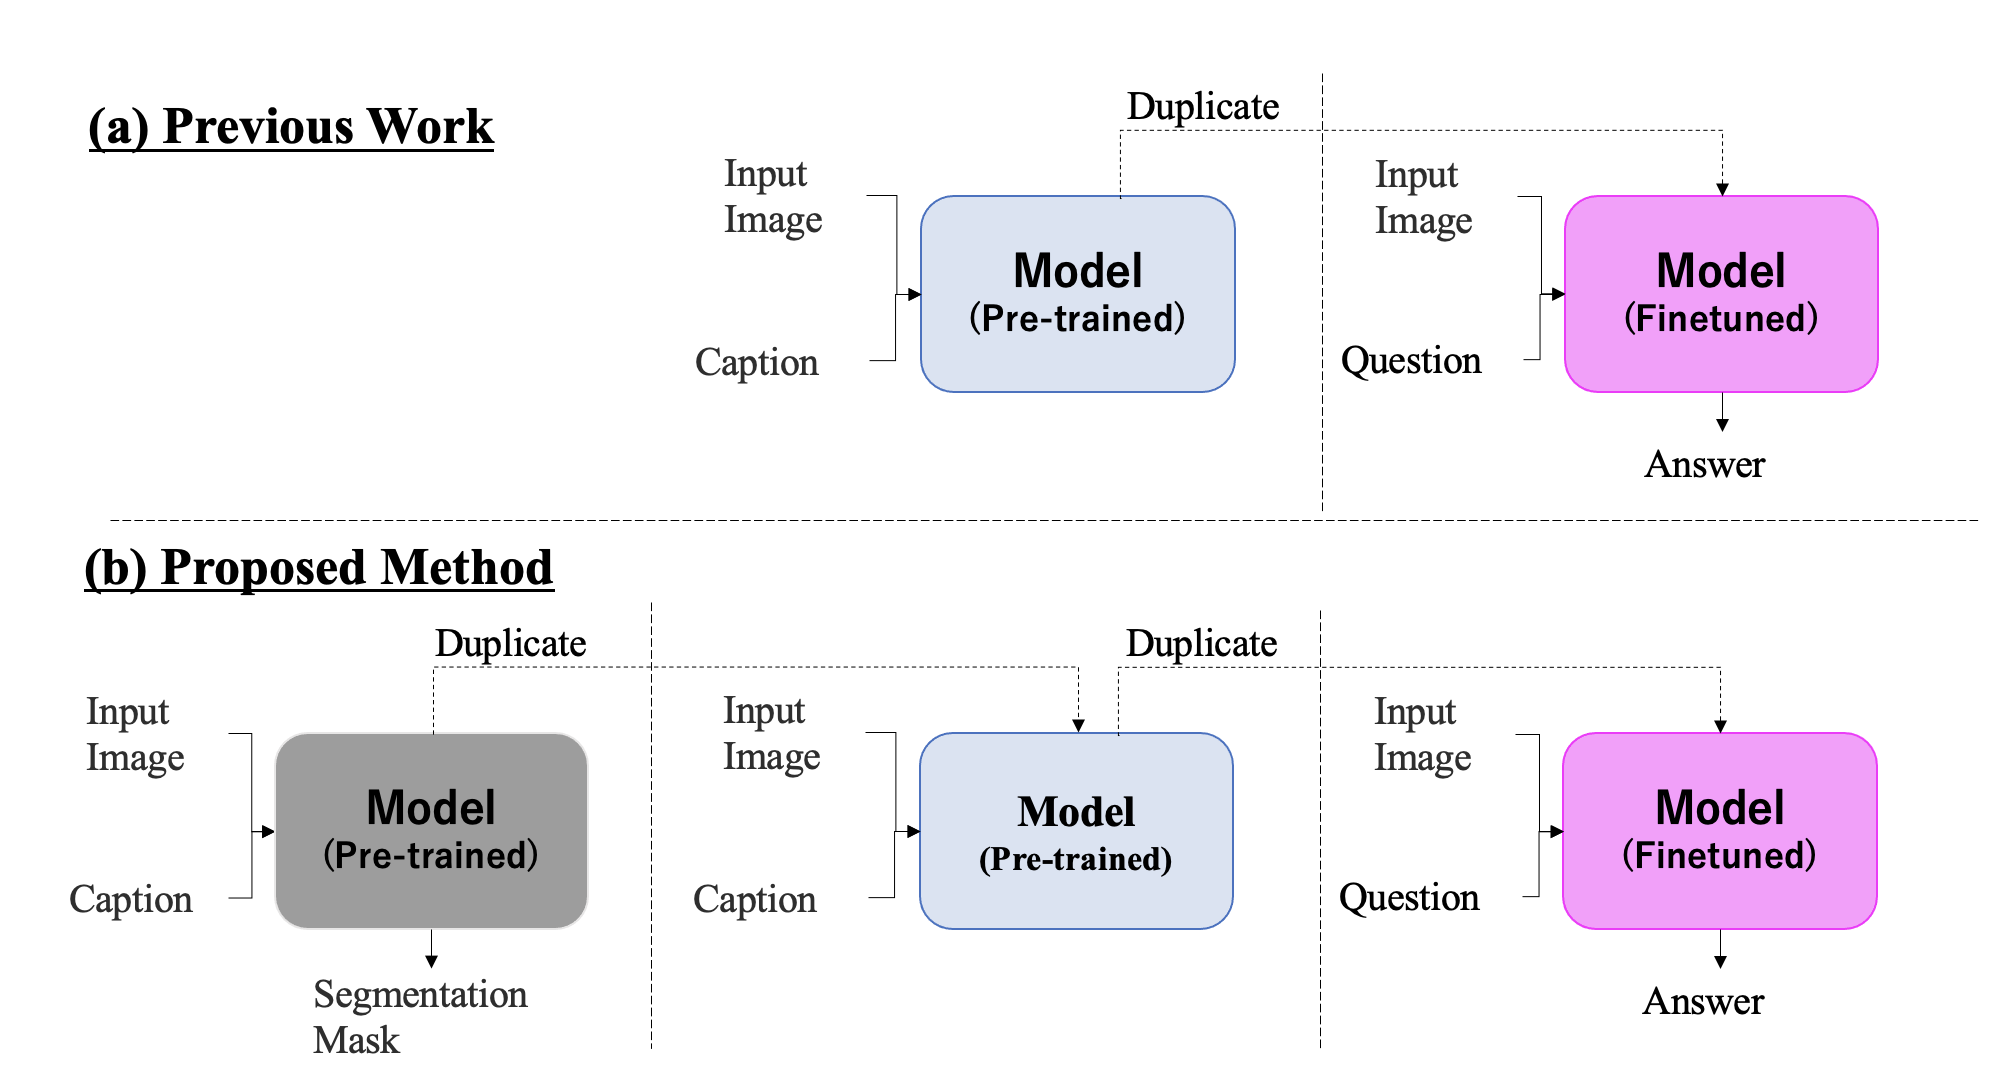
\includegraphics[width=1.0\linewidth]{Chapter_3/chap3_compare.png}
\end{center}
   \caption{Comparative of training pipelines: Previous Work (a) versus Proposed Method (b)
}
\label{fig:compare}
\end{figure}

\subsection{Pre-training Stage One}
\label{Stageone}
During the first stage of pre-training, we employ the semantic segmentation task to convey localized knowledge to the model. The primary objective of this pre-training stage is to equip the model with fundamental organ-specific knowledge, such as the spatial understanding of organs like the liver and lungs. By combining image and text inputs, the model acquires the ability to perform the segmentation task, enabling it to accurately identify the shape, size, and spatial positioning of organs within the images with the aid of textual information. The inputs to this stage consist of image-caption pairs, while the output produced is the corresponding image segmentation mask. This pre-training stage serves as a crucial foundation for subsequent stages, enhancing the model's understanding of basic organ knowledge.

{\bf Objective Function:}
In the pre-training stage one, the loss function includes two components: the dice loss and the binary cross-entropy loss. These loss functions are computed using the output from the model, which is the predicted image segmentation mask, and the corresponding ground truth mask. 

\subsection{Pre-training Stage Two}
\label{Stagetwo}
In the second stage of pre-training, the main objective is to train the model to acquire a comprehensive understanding of both visual and textual information. During this stage, the model receives both the image and its corresponding caption as input and learns in a self-supervised manner. The goal of this stage is to enhance the model's ability to learn meaningful representations by leveraging the rich associations between images and their captions.

{\bf Objective Function:}
Following previous work \cite{chen2022align, chen2022multi}, two key loss functions are utilized: the masked-language modeling (MLM) loss and the image-text matching (ITM) loss.

\section{Datasets}
\label{Dataset}
{\bf Pre-training Stage One:} We use the CHAOS dataset \cite{kavur2021chaos} as the training data. The CHAOS dataset provides a comprehensive collection of medical images with corresponding segmentation masks, which is essential for the image segmentation task. It is a collection of MRI datasets specifically focused on abdominal organs segmentation. It contains annotations for four abdominal organs: liver, right kidney, left kidney, and spleen. Figure~\ref{fig:chaos} shows an example of the CHOAS dataset. The dataset consists of a total of 1594 images designated for training and 1537 images reserved for testing with 256x256 pixels. These masks provide pixel-level annotations that define the boundaries of the organs in the images. However, as our model relies on both text and image information as input, we face the challenge that the CHAOS dataset lacks text information. To address this, we need to generate text captions for the images present in the dataset. The process of generating these captions will be explained
in section~\ref{Gencaption}.

\begin{figure}[t]
\begin{center}
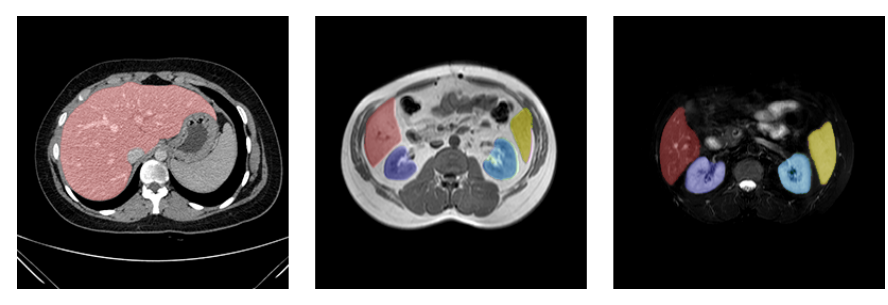
\includegraphics[width=1.0\linewidth]{Chapter_3/chap3_chaos.png}
\end{center}
   \caption{Example images from the CHAOS dataset. It shows CT and MRI images with the liver highlighted in red, right kidney in dark blue, left kidney in light blue, and spleen in yellow.
}
\label{fig:chaos}
\end{figure}

{\bf Pre-training Stage Two:} We use two datasets: the ROCO dataset \cite{Pelka2018RadiologyOI} and the MedICat dataset \cite{subramanian-2020-medicat}. These datasets offer a diverse range of medical images and corresponding text data, allowing the model to further enhance its understanding of visual and textual information.

{\it ROCO dataset:}
This dataset specifically focuses on radiology images and includes over 81,000 image-caption pairs. The images encompass various medical imaging modalities such as Computer Tomography (CT), Ultrasound, X-Ray, and more. Figure~\ref{fig:roco} provides an illustrative example from the ROCO dataset. Figure~\ref{fig:roco2} presents an image along with its associated textual information

{\it MedICat dataset:}
This dataset comprises 217,000 image-caption pairs sourced from 131,000 open access biomedical papers. The dataset offers a diverse range of medical images and associated textual information. Figure~\ref{fig:medicat} shows images and their corresponding captions from the MedICat dataset.
 
{\bf Finetuning:} We use on the SLAKE dataset \cite{liu2021slake}. It offers a wide variety of medical images, accompanied by corresponding questions and answers. It consists of approximately 14,000 samples. The dataset includes a diverse collection of CT and MRI scans, providing a wide range of medical imaging data for training and evaluating our model's performance on the task of medical visual question answering. Figure~\ref{fig:slake} shows an example from the SLAKE dataset.

\begin{figure}[t]
\begin{center}
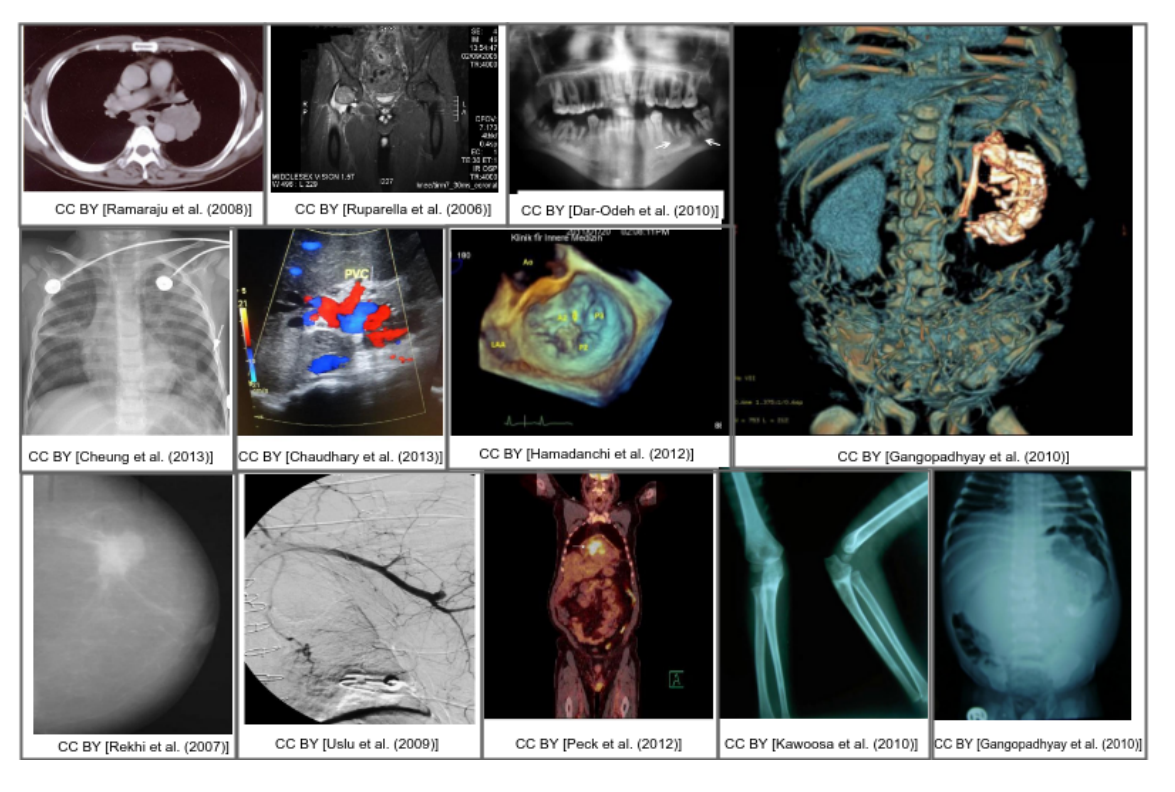
\includegraphics[width=1.0\linewidth]{Chapter_3/chap3_ROCO.png}
\end{center}
   \caption{Example images from the ROCO dataset
}
\label{fig:roco}
\end{figure}

\begin{figure}[t]
\begin{center}
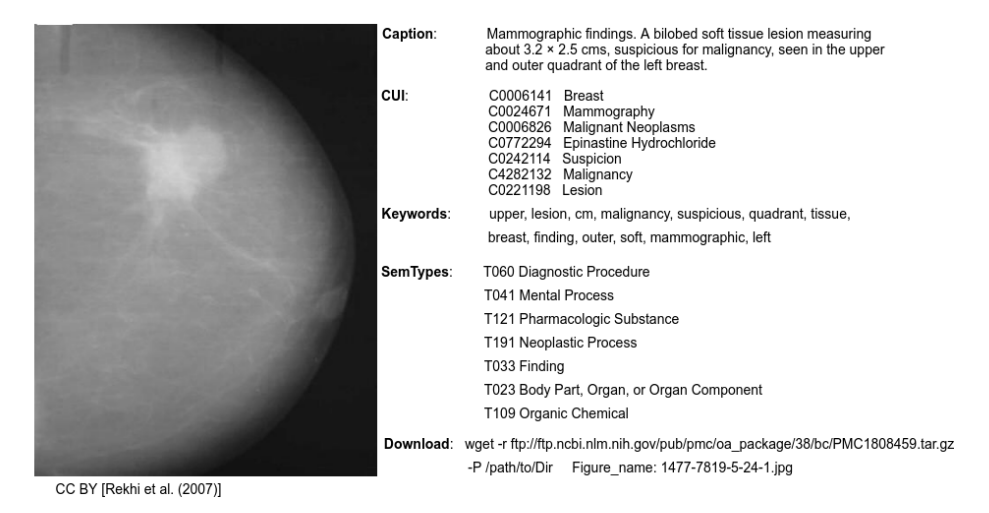
\includegraphics[width=1.0\linewidth]{Chapter_3/chap3_ROCO2.png}
\end{center}
   \caption{An example image and its corresponding caption are obtained from the ROCO dataset. During the pre-training phase, only the images and their corresponding captions are employed.
}
\label{fig:roco2}
\end{figure}

\begin{figure}[t]
\begin{center}
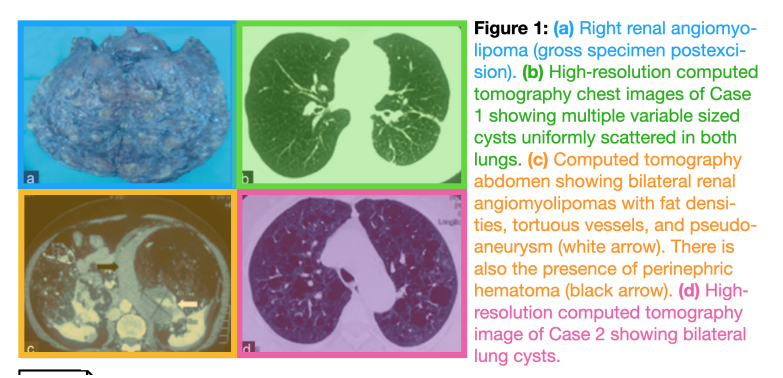
\includegraphics[width=1.0\linewidth]{Chapter_3/chap3_medicat.png}
\end{center}
   \caption{Example images and corresponding captions from the MedICat dataset
}
\label{fig:medicat}
\end{figure}

\begin{figure}[t]
\begin{center}
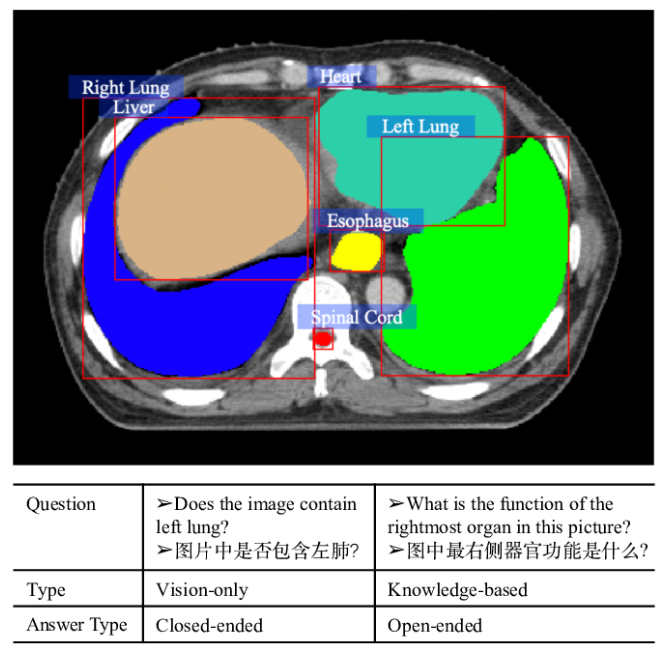
\includegraphics[width=1.0\linewidth]{Chapter_3/chap3_slake.png}
\end{center}
   \caption{An example from the SLAKE dataset is presented. It is worth noting that only English language is used during training.
}
\label{fig:slake}
\end{figure}


\section{Generate Caption Dataset for Pre-training Stage One}
\label{Gencaption}

% However, in the context of the first stage pre-training, existing research lacks a dataset that encompasses both images, segmentation masks, and accompanying text information. Consequently, it becomes imperative for us to generate our own dataset. To accomplish this, we leverage existing medical image segmentation datasets and augment them with the necessary text information. This involves generating text descriptions that are directly related to the corresponding image segmentation masks. By combining these two modalities, we can create a comprehensive dataset that facilitates effective pre-training and aligns with the objectives of our research.
The CHAOS dataset consists of images and their segmentation masks, lacking the textual information necessary for our method. In order to address the requirement of incorporating both image and caption data in the pre-training stage one, it becomes necessary to generate the relevant textual information corresponding to the images. By synergistically integrating these two modalities, our approach effectively facilitates the pre-training process, aligning seamlessly with the core objectives of our research.

We employ the task of generating descriptive captions for the CHAOS dataset as part of our methodology. The process involves using a predefined prompt, "a magnetic resonance imaging of the $[CLASS]$," where $[CLASS]$ represents the class corresponding to the segmentation mask of the image. For instance, if the segmentation mask corresponds to the liver, the generated text would be "a magnetic resonance imaging of the Liver."\; see Figure~\ref{fig:genCaption}. When an image contains multiple organs with their respective segmentation masks, we address this by randomly selecting one organ for each training iteration. Consequently, an image with multiple segmentation masks can yield multiple generated captions. This methodology enables the inclusion of text information that complements the image data during the pre-training stage one.

\begin{figure}[t]
\begin{center}
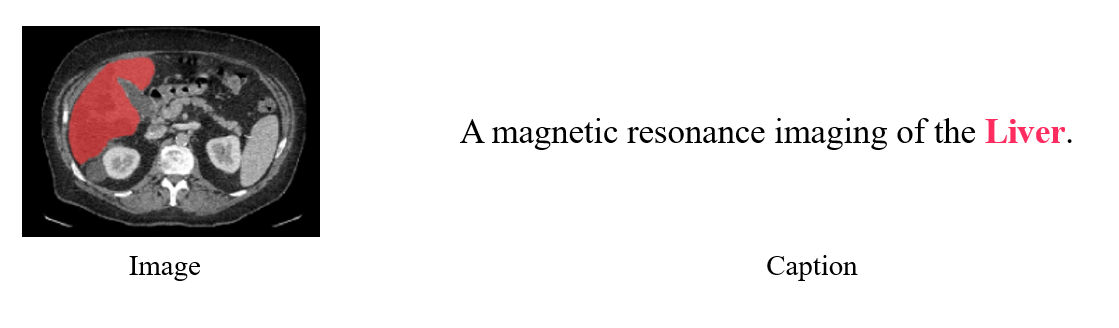
\includegraphics[width=1.0\linewidth]{Chapter_3/chap3_genCaption.png}
\end{center}
   \caption{Medical image segmentation with corresponding generated captions. The component of the image is from paper \cite{kavur2021chaos}.
}
\label{fig:genCaption}
\end{figure}